\section{Event geometry}
\label{sec:eventGeometry}

\subsection{Modeling the Antarctic continent}
Crust 2.0~\cite{crust2} is used to model the Earth's interior near the 
surface.  It is based on seismological data published from the Cooperative Studies of the Earth's Deep Interior (CSEDI).
The model gives thicknesses and densities of seven material
layers in $2^{\circ} \times 2^{\circ}$ bins:  ice, water, soft sediments, hard sediments, upper crust,
middle crust, and lower crust.  

The total Antarctic ice volume is computed by summing the product of ice
thickness and surface area for each bin within the Antarctic continent.
The area of each bin is calculated following:
\begin{equation}
\int_{\phi_1}^{\phi_2}\int_{\theta_1}^{\theta_2}\sin{\theta}~d\theta~d\phi=\left(\phi_2-\phi_1\right)\times\left(\cos{\theta_1}-\cos{\theta_2}\right) \, ,
\end{equation}
\noindent where the limits of the integrals define the edges of the bin in
latitude and longitude.
It is also possible to run the simulation using BEDMAP ice thickness
and subglacial topographic model of Antarctica, developed by the
British Antarctic Survey~\cite{bedmap}.
This model has a much more accurate representation of the ice in
Antarctica, but it is much slower to run, so by default we use
Crust 2.0.
Using Crust 2.0, the \icemc program finds $2.976 \times 10^{16}$ m$^3$ of Antarctic ice in this model, compared to $3.011 \times 10^{16}$ m$^3$ reported by the US Geological Survey~\cite{usgs}, a 1.15\% difference.

\subsection{Picking interaction point and direction}
\label{sec:pickneutrino}

For each neutrino event, the payload position is chosen at random from a set of positions along the ANITA flight path (see Figure~\ref{fig:ANITA_flightPath}).
To simulate only those neutrino interactions that might lead to a detectable signal, interaction positions are limited to occur within the horizon as seen by the payload (roughly between 700 and 800\,km from the payload), and neutrino directions are chosen from an annulus on the sky consistent with viewing angles detectable at the payload (see Section~\ref{sec:weights}). 
The maximum angle that the ray may diverge from the axis of the Cherenkov cone for the interaction to still be detectable depends on the electric field, the distance from the interaction to the payload, and shower nature: this is typically between 10 and 13 degrees.

Both direct and reflected detection is simulated.
In the first case the signal is propagated from the interaction position upwards to the payload. In the second case, the signal is propagated downwards
towards to the ice-rock interface, approximated as a flat mirror,
where the signal is then reflected upwards towards the payload. 


\subsection{Event weighting}
\label{sec:weights}
To minimize computation time,
each event is weighted according to the probability of the neutrino reaching the interaction point without being absorbed in the earth, as well as
the "phase space" reduction (defined below), such that only those topologies that give measurable signal are fully simulated. 
As a neutrino moves through the earth, it encounters varying
densities as it passes through layers of the earth's interior,
and thus differing interaction lengths. 
The neutrino survival probability is thus calculated from the along-track
water-equivalent amount of material traversed.

The phase space factor is the product of the weights derived from the neutrino interaction position and neutrino direction.
These weights are assumed to be independent of one another.
The position weight arises due to the neutrino interaction position being
chosen only within the payload horizon.
This is calculated as
the ratio of the volume of ice within the horizon for the $i^{th}$
event and the total volume of ice in Antarctica (ratio of the yellow to blue
volumes in Figure~\ref{fig:weights}).
The neutrino direction is chosen such that the axis of the Cherenkov cone
lies close in solid angle to the direction from the interaction point to the payload. 
The direction weight is calculated as the ratio of the solid angle coming from the Cherenkov cone and a unit sphere (see purple cone in Figure~\ref{fig:weights}).


\begin{figure}[!h]\centering
  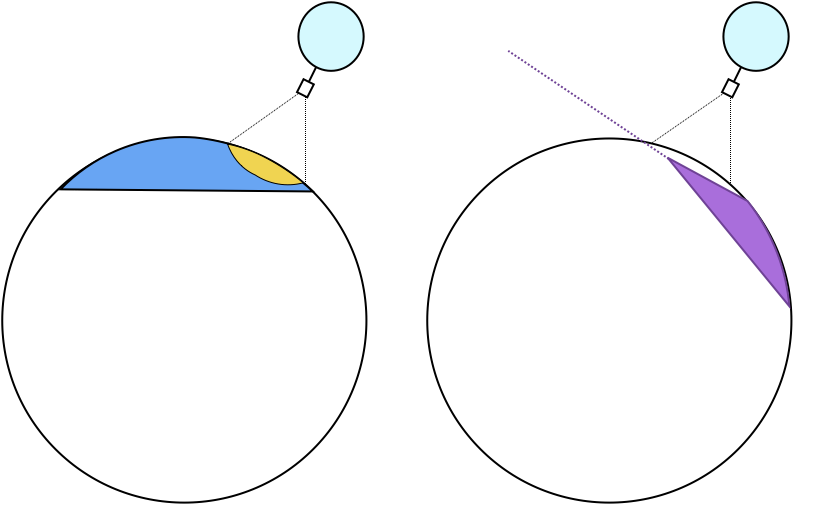
\includegraphics[width=.8\linewidth, trim = 0 6.5cm 0 0, clip]{./Figs/icemcWeightScheme.png}
  \caption{A schematic of the phase space weights used in \icemc. The
    position weight arises because only interaction positions within
    the balloon horizon are simulated (yellow over blue area).
  The direction weight arises because only favourable directions around the
  Cherenkov cone are simulated (purple angle over a unit sphere).}
  \label{fig:weights}
\end{figure}
